% Define document class
\documentclass[twocolumn]{aastex631}
\usepackage{showyourwork}
\usepackage[ruled,vlined,linesnumbered]{algorithm2e}
\usepackage{algorithmic}
\usepackage{color}

\definecolor{rb4}{HTML}{27408B}
\newcommand{\kw}[1]{{\color{rb4}[KW: #1 ]}}
\definecolor{pyRed}{RGB}{214, 39, 40}
\newcommand{\te}[1]{\textbf{\color{pyRed}(TE: #1)}}

\newcommand{\flatiron}{\affiliation{Center for Computational Astrophysics,
Flatiron Institute, New York, NY 10010, USA}}
\newcommand{\jhu}{\affiliation{William H. Miller III Department of Physics and Astronomy, Johns Hopkins University, Baltimore, Maryland 21218, USA}}

\SetKwInput{Parameters}{Parameters}
\SetKwInput{Variables}{Variables}

% Begin!
\begin{document}

% Title
\title{Turbo fast no compromise gravitational wave parameter estimation}
% Title Options
% \title{Ripples in the Flow: \\ Fast, General Parameter Estimation with Normalizing Flows and Differentiable Waveforms}

% Author list
\author{Kaze W. K. Wong}
\email{kwong@flatironinstitute.org}
\flatiron

\author{Maximiliano Isi}
\flatiron

\author{Thomas D. P. Edwards}
\jhu

% Abstract with filler text
\begin{abstract}
We present a light-weighted, flexible, and high-performance framework to
estimate gravitational wave event parameters. By combining heterodyned
likelihood, automatically differentiable and accelerators compatible waveforms,
normalizing flow enhanced gradient-based Markov Chain Monte Carlo (MCMC), we
achieve parameter estimation for real events like GW150914 and GW170817 within a
minute of sampling time. Our framework does not require pre-training or explicit
reparameterization and can be generalized to handle higher dimensional problems.
We also discuss as near real-time parameter estimation has been shown to be
possible by multiple groups, what are the trade-offs and future developments the
community should be aware of. Our code for generating the manuscript and running
the analysis is publically available on GitHub.
\end{abstract}

% Main body with filler text
\section{Introduction}
\label{sec:intro}

% Brief description of PE
Parameter estimation (PE) is one of the most commonly performed data analysis
tasks in gravitational wave (GW) data analysis. The central question of PE is to
infer the parameters of a particular GW model given the strain data. In the
standard compact binary coalescence scenario, this could mean inferring
intrinsic parameters such the masses and spins of the event, as well as
extrinsic parameters such as sky localization and distance from Earth to the
event. PE is also used in testing general relativity (GR), which the main
question is then to check for deviations in parameters that are related to
non-GR modifications \kw{cite}. PE is a crucial step in GW science, since it translate
characteristics of the strain data into astrophysically relevant quantities that
can be used to constrain astrophysical phenomenon such as theories of binary
evolution \kw{cite}.

% Old codes have trouble handling next gen data
The PE results in the most recent catalog of GW events are powered by several
community-developed PE codes, including \texttt{lalinference}, \texttt{pycbc},
and \texttt{bilby} \cite{Romero-Shaw:2020owr} \kw{cite}. These packages have
been tested by a number of groups and are well regarded as the standard tools.
While the standard tools have passed many robustness tests, they are known to be
computationally intensive. The exact amount of time needed to analyze one event
depends on the length of the event. These community tools take about a week to
analyze shorter events such as binary black hole (BBH) mergers, whereas they can
take up to a month on a computer cluster to analyze longer events such as binary
neutron star (BNS) mergers. In the coming decade, there are planned upgrade for
existing facilities and next-generation detector such as the Einstein Telescope
(ET) \kw{cite} and the Cosmic Explorer (CE) \kw{cite}. These upgrades will
increase the sensitivity of the detectors and allow for the detection of more
events with better signal-to-noise ratio (SNR). The number of events that will
be detected in the coming decade is expected to grow from around a thousand per
year to over a million per year. This will put a significant strain on the
current PE tools, which are not designed to handle this many events.

% Effort going to new tools development.
In order to handle the future catalog, there are efforts from multiple groups
developing tools to speed up the PE process. This includes methods that employ
modern tools such as deep learning-based method pre-trained on a large
collection of waveforms \kw{cite}, as well as methods that simplify the
computational challenge by leveraging our knowledge about GW signals \kw{cite}.
While these methods are promising avenues to tackle standard GW analysis tasks
in the coming decade, particularly about events involving compact binary coalescence
(CBC) in GR, they capitalize assumptions that may not be valid for analysis involving
outliers and beyond-GR analysis.

%Basic idea and unique advantage of our tool

In this work, we present a light-weighted, flexible, and high performance
framework to estimate GW event parameters. Our framework implements the
following major features to achieve its performance:
\begin{enumerate}
\setlength{\itemsep}{0pt}
\item Differential waveform models
\item Normalizing flow enhanced MCMC sampler
\item Heterodyned likelihood
\item Native support for accelerator
\end{enumerate}
The main advantage of our framework is it does not rely on specific models or
assumptions about the problem to achieve its performance. This makes our method
extensible to problems beyond the standard CBC analysis. 

%Structure of paper

The rest of the paper is structured as follows: We review the basics of PE and
introduce our framework in section \ref{sec: PE}. We present benchmarking
results on both simulated and real data in section \ref{sec: Result}. Finally,
we discuss the implications of this work and directions for future development
in section \ref{sec: Discussion}.

\section{Gravitational wave parameter estimation}
\label{sec: PE}

\subsection{Likelihood function}
\label{sec:likelihood}

The main objective in PE can be summarized as given data in the form of a time
series of strain $\mathbf{d}$, find the distribution of the source parameters
$\mathbf{\theta}$ that is compatible with the data, i.e.
$p(\mathbf{\theta}|\mathbf{d})$. To compute this object, we can rewrite
it using Bayes' theorem,
\begin{align}
    p(\theta| d) = \frac{\mathcal{L}(d|\theta)\pi(\theta)}{p(d)},
\end{align}
where $\mathcal{L}(d|\theta)$ is the likelihood function, $\pi(\theta)$ is the
prior distribution, and $p(d)$ is the evidence. Since the evidence is a
normalization constant that does not depend on the source parameters, it is
often omitted if we are only interested in the posterior distribution. The prior
distribution is often chosen to be some simple distribution, such as uniformly
distributed in the component masses or a Gaussian distribution in the spins.
Assuming the noise follows from a stationary Gaussian process, the
log-likelihood in the case of GW is given by
\begin{align}
    \log{\mathcal{L}(d|\theta)} = -\left<d-h(\mathbf{\theta})|d-h(\mathbf{\theta})\right>/2,
\label{eq: loglikelihood}
\end{align}
where $d$ is the strain data, $h(\mathbf{\theta})$ is the strain predicted by a
waveform model with a specific set of source parameters. The right hand side of
eq. \ref{eq: loglikelihood} can be evaluated in either time or frequency domain.
Since it is computationally cheaper to compute the likelihood in the frequency
domain, we choose to compute the likelihood throughout this work, which can be defined as 
\te{Need to take the real part?}
\begin{align}
    % \left<a|b\right> = 4 Re\int \frac{a^*(f)b(f)}{\mathcal{S}_n(f)} df,
    \left<a|b\right> = 4 \int \frac{a^*(f)b(f)}{\mathcal{S}_n(f)} df,
\label{eq: innerproduct}
\end{align}
where $\mathcal{S}_n(f)$ is the noise power spectral density (PSD). To compute
the integral shown in eq. \ref{eq: innerproduct}, we need to evaluate a chosen
waveform model $h(\mathbf{\theta})$ at a number of frequnecy sample points.
Evaluating the likelihood function is often the most computationally intensive
part of the PE. The most accurate waveform model is numerical relativity (NR).
However, depending on the source parameters, generating one time series of
strain can take a day to half a year, which makes NR prohibitively
expensive for PE. To circumvent this problem, there are several waveform
"approximant" families, including the IMRPhenom family \kw{}, SEOB family \kw{},
and NR surrogate family\kw{cite}. For shorter events such as a $30-30\ M_{\odot}$
BBH, one waveform call could take $10\text{ms}$ to $\sim 1s$ \kw{verify number
in lalsuite}. For longer events such as a $1.4-1.4\ M_{\odot}$ BNS event, the
evaluation time could go up to \kw{Fill}. Since one needs to evaluate the
likelihood many times during sampling\footnote{A typical PE run with
\texttt{Bilby} takes $>10^6$ likelihood evaluation to converge.}, the
computational cost in evaluating the waveform accumulate and is the main reason
of the long runtime of GW PE.

\subsection{Heterodyned likelihood}

Since the computational cost of evaluating a waveform model scales linearly with
the number of sample points either in the time or frequency domain, the
computational burden for longer-duration signals is often quite large. To
reduce the computational cost, there are a number of methods to reduce the
number of basis points one would need to compute the likelihood faithfully
\kw{cite}. We use heterodyned likelihood \kw{cite} (also named relative binning
in \kw{cite}) in this work. The idea behind heterodyned likelihood can be
summarized as the following: the integrand in eq. \ref{eq: innerproduct} is
a highly oscillatory function, so one has to sample the integrand with
sufficiently dense sampling to compute the integral faithfully. The number of
sample points needed would be much smaller if the integrand was smooth. Given a
pair of waveform parameters $\mathbf{\theta}$ and $\mathbf{\theta_0}$ that are
close to each other, the waveforms generated using the pair of parameters are
similar to each other, this means the ratio between the waveforms is a smoothly
varying function. Given a reference waveform $h(\mathbf{\theta_0})$, we can
exploit this similarity between waveforms to reduce the number of sample points
needed to compute the likelihood for the set of $\mathbf{\theta}$ that is
similar to $\mathbf{\theta_0}$. We decompose the integrand into two parts: a
highly oscillatory part that depends only on the reference waveform and the
data, hence it only needs to be evaluated once; and a smoothly varying part that
depends on the target waveform parameters $\theta$, that needs to be evaluated
for every new likelihood evaluation. Because the part that depends on the target
waveform parameters is smooth, we can use far fewer sample points to compute the
integral with sufficient accuracy.

One may be concerned by the accuracy of this approximation over the target
parameter space, especially in the region where the generated waveform is
significantly different from the reference waveform. However, given we are
interested in the most probable set of parameters, if we choose the reference
waveform to be close to the data, the waveforms that are different from the
reference waveform should also differ significantly from the data. This means
the likelihood value for these waveforms should be significantly smaller than
the likelihood of the waveforms that are similar to the reference waveform,
hence will not be relevant for the PE result. In practice, one will first
optimize the likelihood function with full frequency resolution to obtain the
reference waveform parameters, which can be run at a much lower cost compared to
PE. 

We give a concise description of what we implement
in our code here. For a more extensive derivation of heterodyned
likelihood, we refer the reader to the reference \cite{Zackay:2018qdy}.
In the heterodyned likelihood framework, the two terms in eq \ref{eq:
loglikelihood} are given by
\begin{align}
    \langle d|h \rangle &\approx \sum_b A_0(b) r^*_0(h,b) + A_1(b) r^*_1(h,b), \nonumber \\
    \langle h|h \rangle &\approx \sum_b B_0(b) |r_0(h,b)|^2 + 2 B_1(b) \Re[r_0(h,b)r_1(h,b)],
\label{eq: heterodynedlikelihood}
\end{align}

where $b$ denotes the index of a \textit{sparse} set of bins where the integrand
will be computed on, $A_0(b)$, $A_1(b)$, $B_0(b)$, and $B_1(b)$ are the
heterodyning coefficients computed using the data and the reference waveform,
and $r_0(h,b)$ and $r_1(h,b)$ are the ratio between the target waveform and the
reference waveform at the center of the bin. To evaluate eq. \ref{eq:
heterodynedlikelihood}, we need to be able to first choose a binning scheme,
then evaluate the coefficients given the data and the reference waveform and the
ratio between the target waveform and the reference waveform at the center of
the bin.

Considering the phasing of a waveform is denoted by a power series $\Psi(f) =
\sum_i \alpha_i f^{\gamma_i}$, where $\alpha_i$ are some coefficients depending
on the waveform parameters and $\gamma_i$ are powers motivated by post-Newtonian
theory. For example, for the term $\gamma_i = -5/3$, $\alpha_i$ is related to
the chirp mass. The maximum dephasing one can have within a frequency interval $[f_{\textrm{min}},f_{\textrm{max}}]$ is given by
\begin{align}
    \delta \Psi_{\textrm{max}}(f) = 2\pi \sum_{i} (f/f_{*,i})^{\gamma_i} \textrm{sgn}(\gamma_i),
\label{eq: maxdephasing}
\end{align}
where $f_{*,i} = f_{\textrm{max}}$ for $\gamma_i>=0$ and $f_{*,i} =
f_{\textrm{min}}$ for $\gamma_i<0$. Given the relation shown in eq. \ref{eq:
maxdephasing}, we can choose the binning scheme which divide the entire
frequency domain of interests into a set of bins such that the maximum dephasing
within each bin is smaller than a certain threshold $\epsilon$, i.e.
$|\delta\Psi_{\textrm{max}}(f_{\textrm{max}}) -
\delta\Psi_{\textrm{max}}(f_{\textrm{min}})| < \epsilon$. 

Given a sufficiently dense binning scheme, the ratio between the target waveform
and the reference within a bin can be approximated by linear interpolation
\begin{align}
r(f) = \frac{h(f)}{h_0(f)} = r_0(h,b) + r_1(h,b)(f- f_m(b)) + \cdots,
\label{eq:definer}
\end{align}
where $b$ is the index of a particular bin, $r_0(h,b)$ and $r_1(h,b)$ are the
value and slope of the ratio at the center of the bin respectively, and
$f_m(b)$ is the center frequency of the bin. Since we have access to both $h(f)$
and $h_0(f)$, we can compute $r_0$ and $r_1$ by evaluating the value of $r(f)$
at the edge of the bin and invert eq. \ref{eq:definer}.

The final ingredient we need is the heterodyning coefficients given the data and
the reference waveform on the sparse bins, which are given by
\begin{align}
    A_0(b) &= 4 \sum_{f \in b} \frac{d(f)h^*_0(f)}{S_n(f)} df, \\
    A_1(b) &= 4 \sum_{f \in b} \frac{d(f)h^*_0(f)(f-f_m(b))}{S_n(f)} df, \\
    B_0(b) &= 4 \sum_{f \in b} \frac{|h_0(f)|^2}{S_n(f)} df, \\
    B_1(b) &= 4 \sum_{f \in b} \frac{|h_0(f)|^2(f-f_m(b))}{S_n(f)} df.
\end{align}
Note that the sum within each bin should be done with the same sampling rate as
the data, i.e. the same one would do in the case without using heterodyned
likelihood.

\te{Do we also already here want to make the point that it really helps with memory issues of GPUs if the frequency array isn't too large?}

\subsection{MCMC with Gradient-based sampler}
\label{sec:gradient}

Given eq. \ref{eq: loglikelihood} and the prior, one can evaluate the posterior
density function over the entire parameter space of interest to obtain the most
probable set of points that are consistent with the data. However, direct
sampling quickly becomes intractable as the dimensionality of the parameter
space increases beyond a few dimensions. Markov chain Monte Carlo (MCMC) is a
common method employed to generate samples when direct sampling is not possible.

In MCMC, the posterior distribution is approximated by a Markov chain that
converges to the target distribution. The Markov chain is constructed by
iteratively proposing a new point in the parameter space based on the current
location of the chain. The proposed point is accepted with a probability that is
usually set to be proportional to the ratio of the posterior density evaluated
at the proposed point and the current point. The chain can either accept the
proposal and move to the new location or reject the proposal and stay at the
current location. This process is repeated until the chain converges to the
target distribution. The samples generated by the chain are then used to
estimate the quantities of interest, such as the mean and credible intervals of
the source parameters. In practice, since we do not know the target distribution
ahead of time, the MCMC process is usually repeated until a certain criterion is
met, such as a Gelman-Rubin convergence statistic \cite{Gelman-rhat} lower than
a threshold or simply after a certain number of iterations.

Compared to direct sampling, MCMC algorithms only explore regions that are
highly probable, thus reducing the computational cost by not wasting resources in
regions where it is unlikely to generate the data. However, MCMC algorithms come
with their own set of issues. To illustrate what difficulties an MCMC algorithm
may face, we can examine one of the most vanilla MCMC algorithm, the
Metropolis-Hastings algorithm with a Gaussian kernel. Starting at some initial
point, one can draw a proposed point from a Gaussian transition kernel, defined
as
\begin{align}
    q(\mathbf{x},\mathbf{x_0})= \mathcal{N}(\mathbf{x}|\mathbf{x_0},\mathbf{C}),
\end{align}
where $\mathbf{x_0}$ is the current location of the chain, $\mathbf{x}$ is the
proposed location, and $\mathbf{C}$ is the covariance matrix of the Gaussian. In
the simplest case, we can pick $\mathbf{C}$ to be a diagonal matrix with a
constant value, which corresponds to an isotropic Gaussian center around the
current location with a constant variance. And the acceptance criteria is
defined as
\begin{align}
\alpha(\mathbf{x},\mathbf{x_0}) = \min\left(1,\frac{p(\mathbf{x})q(\mathbf{x_0},\mathbf{x})}{p(\mathbf{x_0})q(\mathbf{x},\mathbf{x_0})}\right).
\label{eq:Gaussian_acceptance}
\end{align}

We can see from eq. \ref{eq:Gaussian_acceptance} the acceptance rate is
proportion to the fraction of volume where the posterior density at the proposed
location is higher than the current location within the Gaussian transition
kernel. If we choose the variance of the transition kernel to be too large, this
fraction will be small hence the acceptance rate will be poor. On the other
hand, if one chooses the variance to be too small, nearby samples will be
correlated. In both cases, the efficiency in constructing the chain with a
target number of independent samples is suboptimal. There is often a tuning
process before we run the MCMC algorithm to find the optimal tuning parameters,
in this example the variance of the Gaussian, to ensure close to optimal
performance.

However, as we are dealing with higher dimensional problems, even the optimally
tuned Gaussian transition kernel does not guarantee good performance. In order
to have a reasonable acceptance rate, the variance of the Gaussian has to be
smaller in a higher dimensional space, which means the transition kernel is in
general making smaller and smaller steps as we increase the dimensionality.

Transition kernels that leverage gradient information of the target
distribution can help to address this issue of shortening steps in a high
dimensional space. Instead of proposing a new point by drawing from a Gaussian,
one can use the gradient evaluation at the current location to propose a new
point. For example, Metropolis-adjusted Langevin algorithm (MALA) \kw{cite}
place a unit Gaussian at the tip of the gradient vector at the current position,
\begin{align}
    \mathbf{x} = \mathbf{x_0} + \tau \nabla\log{p(\mathbf{x_0})} + \sqrt{2\tau}N(0,\mathbf{I}),
\end{align}
where $\tau$ is the step size, which is a tuning parameter. Compared to a
Gaussian centers at the current location, the MALA transition kernel is more
likely to propose a point into the higher posterior density region because of
the gradient term, which helps to boost the acceptance rate.

While transition kernels that use gradient information can help to improve the
acceptance rate, computing the gradient of the posterior density function
introduce additional computational cost, which is not necessarily beneficial in
terms of sampling time. If one wants to compute the gradient information through
finite differencing, the additional computation cost goes as at least $\sim
\mathcal{O}(2n)$, where $n$ is the dimension of the problem. \texttt{Jax} allows
us to compute the gradient of the likelihood function with respect to the
parameters through automatic differentiation, which gives the gradient
information down to machine precision at around the same order of time compared
to evaluating the posterior itself. Having access to gradient information
through automatic differentiation is crucial to make the trade-off between using
gradient-based transition kernels and additional computation cost favorable.

\subsection{Normalizing Flow enhanced sampling}
\label{sec:flow}

% Problem with just HMC or MALA
While gradient-based samplers have been shown to be superior in terms of
performance when compared to other gradient-free algorithms in many practical
examples\kw{cite}, there are still a number of classes of problems
gradient-based samplers do not solve well. \footnote{To be specific, we are
referring to sampling algorithms that use first-order derivatives here. Sampling
algorithms that use the information of higher order derivatives such as manifold-MALA
and Riemannian-HMC can in principle decorrelate local correlation in the target
distribution, however, they often have instability issues when they are used on
real-life applications, so they are not used often in practice.} For example,
target distribution that exhibits local correlation is hard to deal with,
since by construction first order gradient-based algorithms can only handle
global correlation structure. Another example is multi-modality. If there are
multiple modes in the target distribution, an independent chain will likely 
be trapped in one mode and take an extremely long time to transverse between the
modes. This means the relative weights between modes will much longer to sample
compared to the shape of each mode.

% Long burn-in too
Moreover, before we can use the sampling chain to estimate the quantity we care about,
the sampler often needs to first find the most probable region in the target
space, which is a common process that is referred to as "burn-in" in the
literature. This means one would discard a certain amount of data generated from
the beginning and only use the later part to estimate the quantities of
interest. The burn-in phase of a gradient-based sampler is often as long as the
sampling phase, which means a good portion of computation is not necessarily
helpful in estimating the target quantities.

% Crux of normalizing flow
Normalizing flow is a neural-network based technique that aims at learning a
mapping between a simple distribution, such as a Gaussian distribution, to a
complex distribution, often given in the form of data samples from a target
distribution. Once the network is trained, one can evaluate the probability
density of the complex distribution and samples from it very efficiently.
The core of normalizing flow is given by
\begin{align}
    p_x(X) = p_z(Z) \left| \frac{\partial f}{\partial z}\right|,
\end{align}
where $p_x(X)$ is the complex target distribution $p_z(Z)$ is the simple latent
distribution and $f$ is an invertible parameterized transform that
connect the two distributions. For a detailed discussion of the algorithm, we
refer the readers to \kw{cite}.

% The flowMC algorithm
As mentioned in the previous subsection, one of the main issue gradient-based
sampler is it does not explore locally correlated features and multi-modality well. This
is exactly where the normalizing flow model can help. Once multiple independent
chains have generated samples, we can combine the samples and feed them to the
normalizing flow, which learns the global landscape of the target
distribution. Note that since the independent chains are generated with the same
number of samples, the normalization between posterior density represented by
different chains is in general different from the true target distribution. To
adjust for this inaccuracy, we use the normalizing flow model as a
\textit{proposal} distribution. Given a trained normalizing flow model, we can
generate the proposed jump in the target space by sampling from the latent
distribution $z \sim p_z(Z)$, then push it through the learned map given by the
normalizing flow model $x=f(z)$. the acceptance criteria is given by
\begin{align}
    \alpha(\mathbf{x},\mathbf{x_0}) = \min \left[ 1, \frac{\hat{\rho}(\mathbf{x_0})\rho_*(\mathbf{x})}{\hat{\rho}(\mathbf{x})\rho_*(\mathbf{x_0})}\right],
\end{align}
where $\hat{\rho}$ is the probability density estimated by the normalizing flow
model, $\rho_*$ is the probability density evaluated using the target function,
and $x_0$ is the current position. We can see the flow distribution is the
target distribution when the accepting probability is 1. When the normalizing
flow model has not converged to the target distribution, only a portion of the
proposed jumps will be accepted. This means an MCMC process using the
normalizing flow model as the proposal distribution can adjust the normalization
across different regions of the target parameter space by rejecting jumps into
less likely regions. The training and sampling are then repeated until certain
criteria are met. Note that every time we retrain the network, we are breaking
the Markov properties since we are changing the proposal distribution. To
produce final samples that can be used to estimate target quantities, one has to
freeze the normalizing flow model and not retrain during the final sampling
phase in order to satisfy the detailed balance condition. To summarize the
sampling process, the pseudocode is given by

\begin{algorithm}
\caption{flowMC pseudocode}\label{alg:cap}
\KwIn{Initial position $ip$}
\Parameters{n training loop $nt$, n production loop $np$}
\Variables{current chain $cc$, current position $cp$, current NF parameters $\Theta$}
\KwResult{Chains}
$cp \leftarrow ip$\\
\tcc{Training loop}
    \For{$i<nt$}{
        $cc, cp \leftarrow LocalSampling(cp)$\\
        $\Theta \leftarrow TuneNF(cc)$\\
        $chains, cp \leftarrow GlobalSampling(cp, \Theta)$ \\
        $cc \leftarrow Append(cc, chains)$
    }
\tcc{Production loop}
    \For{$i<np$}{
        $c_local, cp \leftarrow LocalSampling(cp)$\\
        $c_global, cp \leftarrow GlobalSampling(cp, \Theta)$ \\
        $Chains \leftarrow Append(Chains, c_local, c_global)$
    }

\Return{$Chains$}
\end{algorithm}

% Observation of traits of flowMC
This means independent chains can now jump between modes, or within a single
mode that exhibits complex geometry that cannot be handled only through the
local sampler, which greatly reduces both the burn-in time and sampling time.

While the method would still work when there is only one independent local
sampler chain, this method works much better when we employ a lot of independent
chains because of the increased number of samples available for training. 
\kw{Mention how this helps gravitational wave, gives examples.}

In practice, we find the normalizing flow not only helps jumping betw

\subsection{Accelerators}
\label{sec:accelerators}

Modern accelerators such as GPUs and TPUs are designed to execute large-scale
dense computation. They are often much more cost-efficient than using many CPUs
when it comes to solving problems that can be benefited from parallelization.
The downside of these accelerators compared to CPUs is they can only perform a
more restricted set of operations and are often less performant when they are
dealing with serial problems. Parameter estimation with MCMC is a serial
problem since each new sample generated from a chain depends on the last sample
in the chain. This means naively putting the problem on an accelerator is more
likely to harm the performance instead of improving it.


% More sample helps training normalizing flow
In this work, the use of accelerators provides two independent perks that
tremendously benefit the parameter estimation process. First, using
accelerators allow us to run many independent chains at the same time, which
benefits the training of the normalizing flow. Since we generate the data we use
to train the normalizing flow on the fly, the more independent data we can feed
to the training process, the higher chance the normalizing flow can learn a
reasonable representation of the global landscape of the target distribution. If
we only use a small number of chains, we are limited to the correlated samples
from each chain, so we have to run more sequential steps to get the same amount
of independent data as compared to running more chains, where the former option does
not benefit from parallelization but the latter does. In another word, being
able to use many independent chains help the normalizing flow learn the global
landscape faster in Wall time.

% GPU helps packing a shit ton of waveform evaluation
Another benefit accelerator brings is the parallel evaluation of waveforms. Since
the waveform models being used in PE are approximants, they can be evaluated at
any given time or frequency independent of what has been generated before the
time or frequency. This means predicting the waveform can be trivially
parallelized over frequency. Together with heterodyned likelihood, we can
evaluate the likelihood at $\mathcal{O}(10^7)$ different locations on an Nvidia
A100 GPU. The high throughput of likelihood evaluations unlocks the potential of
the \texttt{flowMC} sampling algorithms.

\section{Result}
\label{sec: Result}
\subsection{Injection-recovery test}

To demonstrate the robustness of our pipeline, we use it to recover the
parameters of a set of simulated signals. We create a set of simulated signals
and inject them into simulated noise, generated under the Gaussian noise
assumption using the designed PSD for every detector. Then we run our pipeline
given the simulated data and determine the credible interval at the true
parameters of the injected signals. Given the set of credible values, we can
check whether the true value lies within a certain credible interval at a
reasonable frequency. If our pipeline is perfect, we should find the true
parameters lie within $x\%$ credible interval $x\%$ of the time, e.g. the true
value should lie within the $50\%$ credible interval $50\%$ of the time. In
other word, the percentiles of the true parameters should be uniformly
distributed. Deviation from this behavior suggests the pipeline is either
over-confident or too conservative. 

% State the distribution of injected population
We sample 1200 events from the following distribution of parameters detailed in
table \ref{tab:parameters}.
The same distribution of parameters are used as the prior in the PE process.
The simulated signals have a 16 seconds segment length,
and we project the signal on the LIGO Hanford, Livingston and Virgo detector.
We used the designed sensitivity curve for each detector to generate the noise \kw{cite}.
We use a minimum frequency cutoff of 30 Hz with a sampling rate of 2048 Hz.

\begin{table*}[hbt!]
    \begin{center}
    \begin{tabular}{ l l l l l }
    \hline
    \hline
    Parameters &  Description & Injection & GW150914 & GW170817\\

    $M_c$ & Chirp mass $[M_\odot]$& $[10, 50]$ & $[10,80]$ & $[1.18,1.21]$ \\
    $q$ & Mass ratio & $[0.5, 1]$ & $[0.125,1]$ & $[0.125,1]$ \\
    $\chi_1$ & Primary dimensionless spin& $[-0.5, 0.5]$ & $[-1,1]$ & $[-0.3,0.3]$ \\
    $\chi_2$ & Secondary dimensionless spin & $[-0.5, 0.5]$ & $[-1,1]$ & $[-0.3,0.3]$ \\
    $d_L$ & Luminosity distance $[\textrm{Mpc}]$ & $[300, 2000]$ & $[0, 2000]^\dag$ & $[1, 75]^\dag$ \\
    $t_c$ & Coalescence time $[\textrm{s}]$& $[-0.5, 0.5]$ & $[-0.1, 0.1]$ & $[-0.1, 0.1]$ \\
    $\phi_c$ & Coalescence phase & $[0, 2\pi]$ & $[0, 2\pi]$ & $[0, 2\pi]$ \\
    $\cos{\iota}$ & Cosine of inclination angle & $[-1, 1]$ & $[-1, 1]$ & $[-1, 1]$ \\
    $\psi$ & Polarization angle & $[0, \pi]$ & $[0, \pi]$ & $[0, \pi]$ \\
    $\alpha$ & Right ascension & $[0, 2\pi]$ & $[0, 2\pi]$ & $[0, 2\pi]$ \\
    $\sin{\delta}$ & Sine of declination & $[-1, 1]$ & $[-1, 1]$ & $[-1, 1]$ \\

    \hline
    \hline
    \end{tabular}
    \caption{Parameters used and the range of prior for the injection-recovery
    test, GW150914, and GW170817. All priors assume a uniform distribution with
    the range tabulated in the table. The coalescence time refers to a shift in
    time around the trigger time. $^\dag$ Instead of uniform in luminosity
    distance, the distance prior used for the GW150914 and GW170817 analysis are
    uniform in comoving distance, with the range denote by the value in the
    table in $\textrm{MPC}$}
    \label{tab:parameters}
    \end{center}
\end{table*}

% Show injection pp plot
The result of this injection-recovery campaign is shown in fig. \ref{fig:ppplot}. We
computed the quantile of which the true value lies for each marginalized
distribution, then plotted the cumulative distribution of these quantiles. The
shadow band denotes the 95\% credible interval drawn from a uniform distribution
with the same number of events. We can see most the injection-recovery result
lies within the band drawn from a uniform distribution, showing our inference
results agree well with a uniform distribution. There is a small deviation from
a uniform distribution for the secondary spin $\chi_2$, which is not too
alarming since we are computing the quantile for 11 parameters. Having one of
them lying briefly outside the 95\% band does not mean the inference is bias.

To quantify how well our result agrees with a uniform distribution, we can
compute the Kolmogorov-Smirnov test p-values for each marginalized distribution.
If the p-value is too low, often chosen to be $0.05$, then it means our result
does not agree with a uniform distribution, hence it could be biased. The
p-values for each marginalized distribution are shown in the legend of fig.
\ref{fig:ppplot}. We can see most of them are well above the $0.05$ threshold,
except for $\chi_2$, which is mildly below the threshold. Once again, assuming
these p-values are drawn from a uniform distribution, given $11$ draws (the
number of parameters in our inference), it is not abnormal to have one of the
parameters lies slightly outside the threshold. To assess whether this is
expected, we can compute the combined p-value for these 11 parameters, which is $0.47$.
This shows our inference pipeline performs properly on simulated data.
Indeed, the accuracy of our inference pipeline is consistent with other works\kw{cite}.

\begin{figure}
    \script{ppplots.py}
    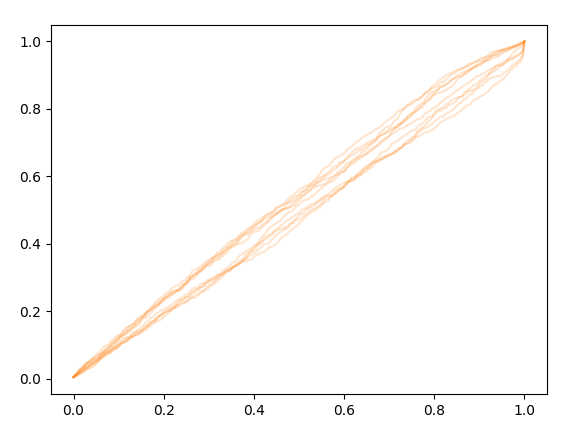
\includegraphics[width=0.99\linewidth]{figures/ppplot.pdf}
    \caption{Cumulative distribution of the quantile of which the true value
    lies for each marginalized distribution. The shadow band denotes the 95\%
    credible interval drawn from a uniform distribution with the same number of
    events as the injection campaign. The legend shows the p-values for each
    marginalized distribution.}
    \label{fig:ppplot}
    \end{figure}

\subsection{Real event parameter estimation}

To demonstrate the performance of our parameter estimation pipeline, we apply
our pipeline to analyze GW150914 and GW170817. The prior used for the two events
are shown in table \ref{tab:parameters}. We use a 4 seconds long segment for the
GW150914 analysis, and a 128 seconds long segment for the GW170817 analysis.
Both data segment are fetched from GWOSC \kw{cite}. Given the specific sampler
setting we use, we produce around an average of 2500 and 3500 \textbf{effective
samples} for GW150914 and GW170817 \footnote{Note that effective sample measures
the number of independent samples, which takes correlation between step into
account, and it is not the same as the number of generated samples. The
effective sample size is computed using
\texttt{arviz},\url{https://python.arviz.org/en/stable/api/generated/arviz.ess.html}.}
in each analysis respectively, which is run on an Nvidia A100 GPU. The
\texttt{wall} time for both event is around 10 minutes. The chain data and the
analysis scripts which generate the chains can be found on
%\kw{\variable{data/} and \variable{script}}
. Most of the time is spent on jit compilation of the code, and the actual
sampling time was about \~150s. Note that we have pre-computed the reference
waveform parameters used in hetetrodyne likelihood for the two events, so the
time spent on solving for the reference waveform parameters is omitted in the
\texttt{wall} time calculation.

\begin{figure}
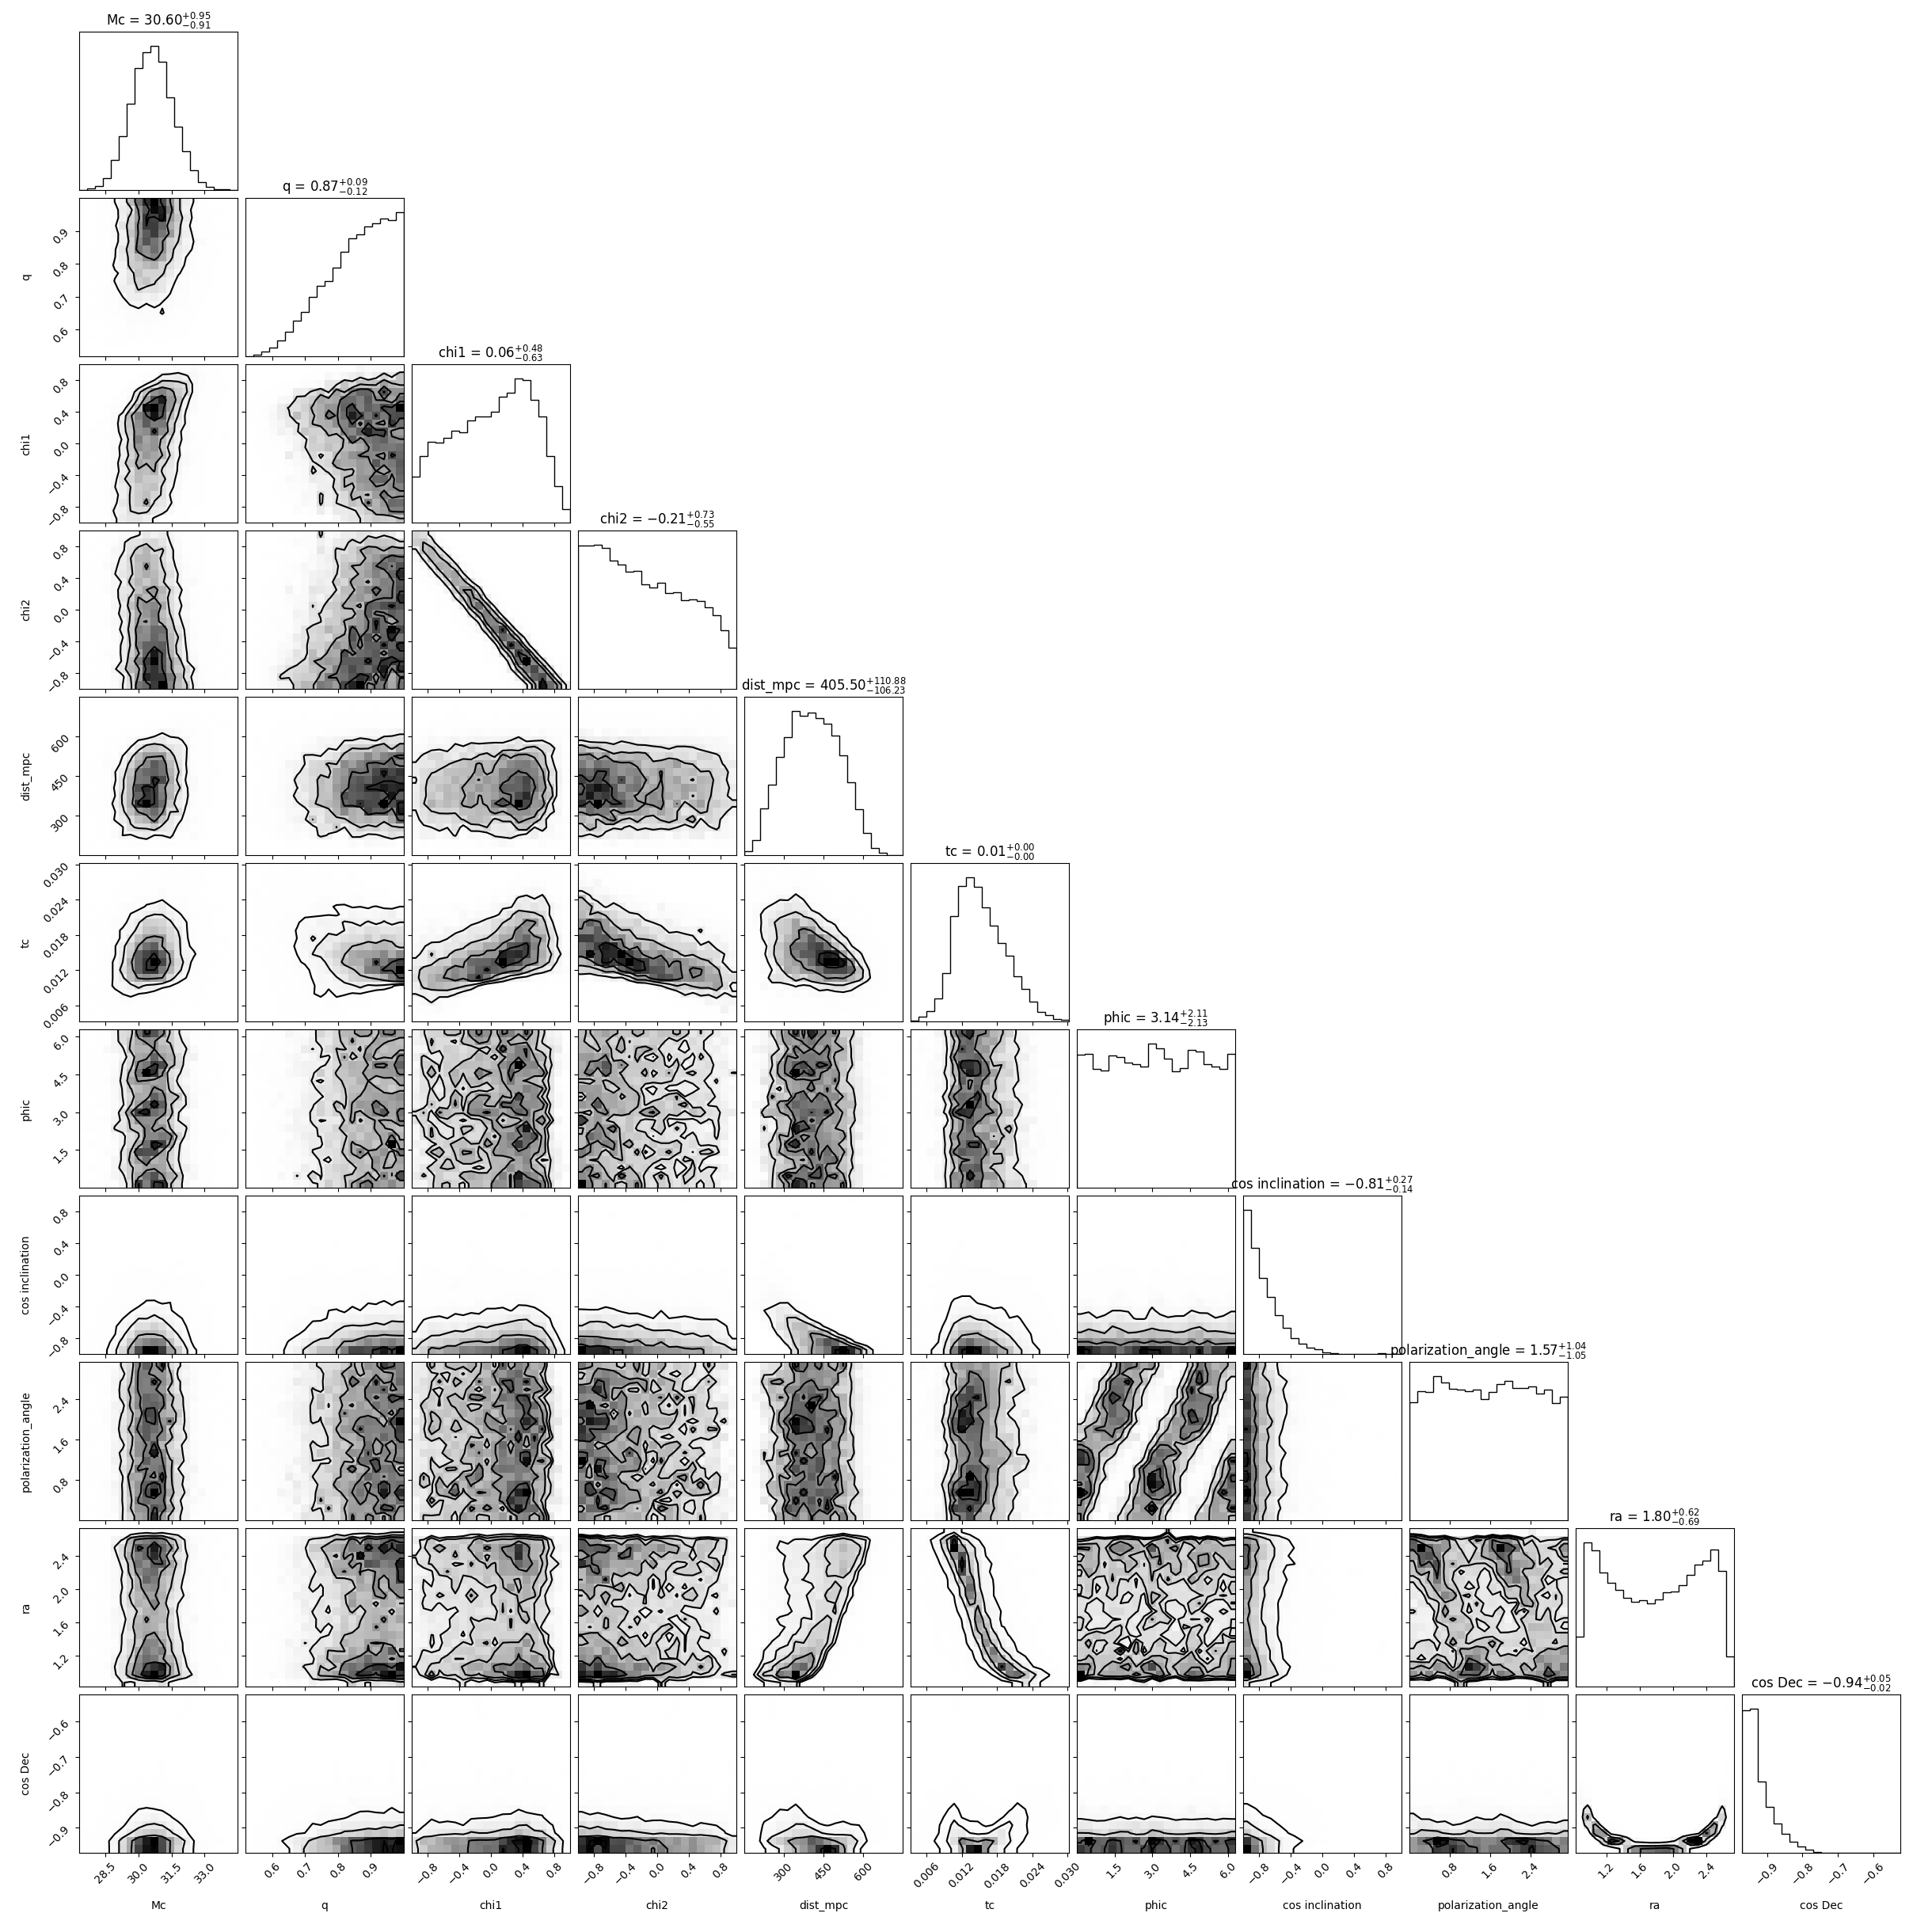
\includegraphics[width=0.99\linewidth]{static/GW150914.png}
\caption{
    hi
}
\label{fig:GW150914}
\end{figure}

\begin{figure}
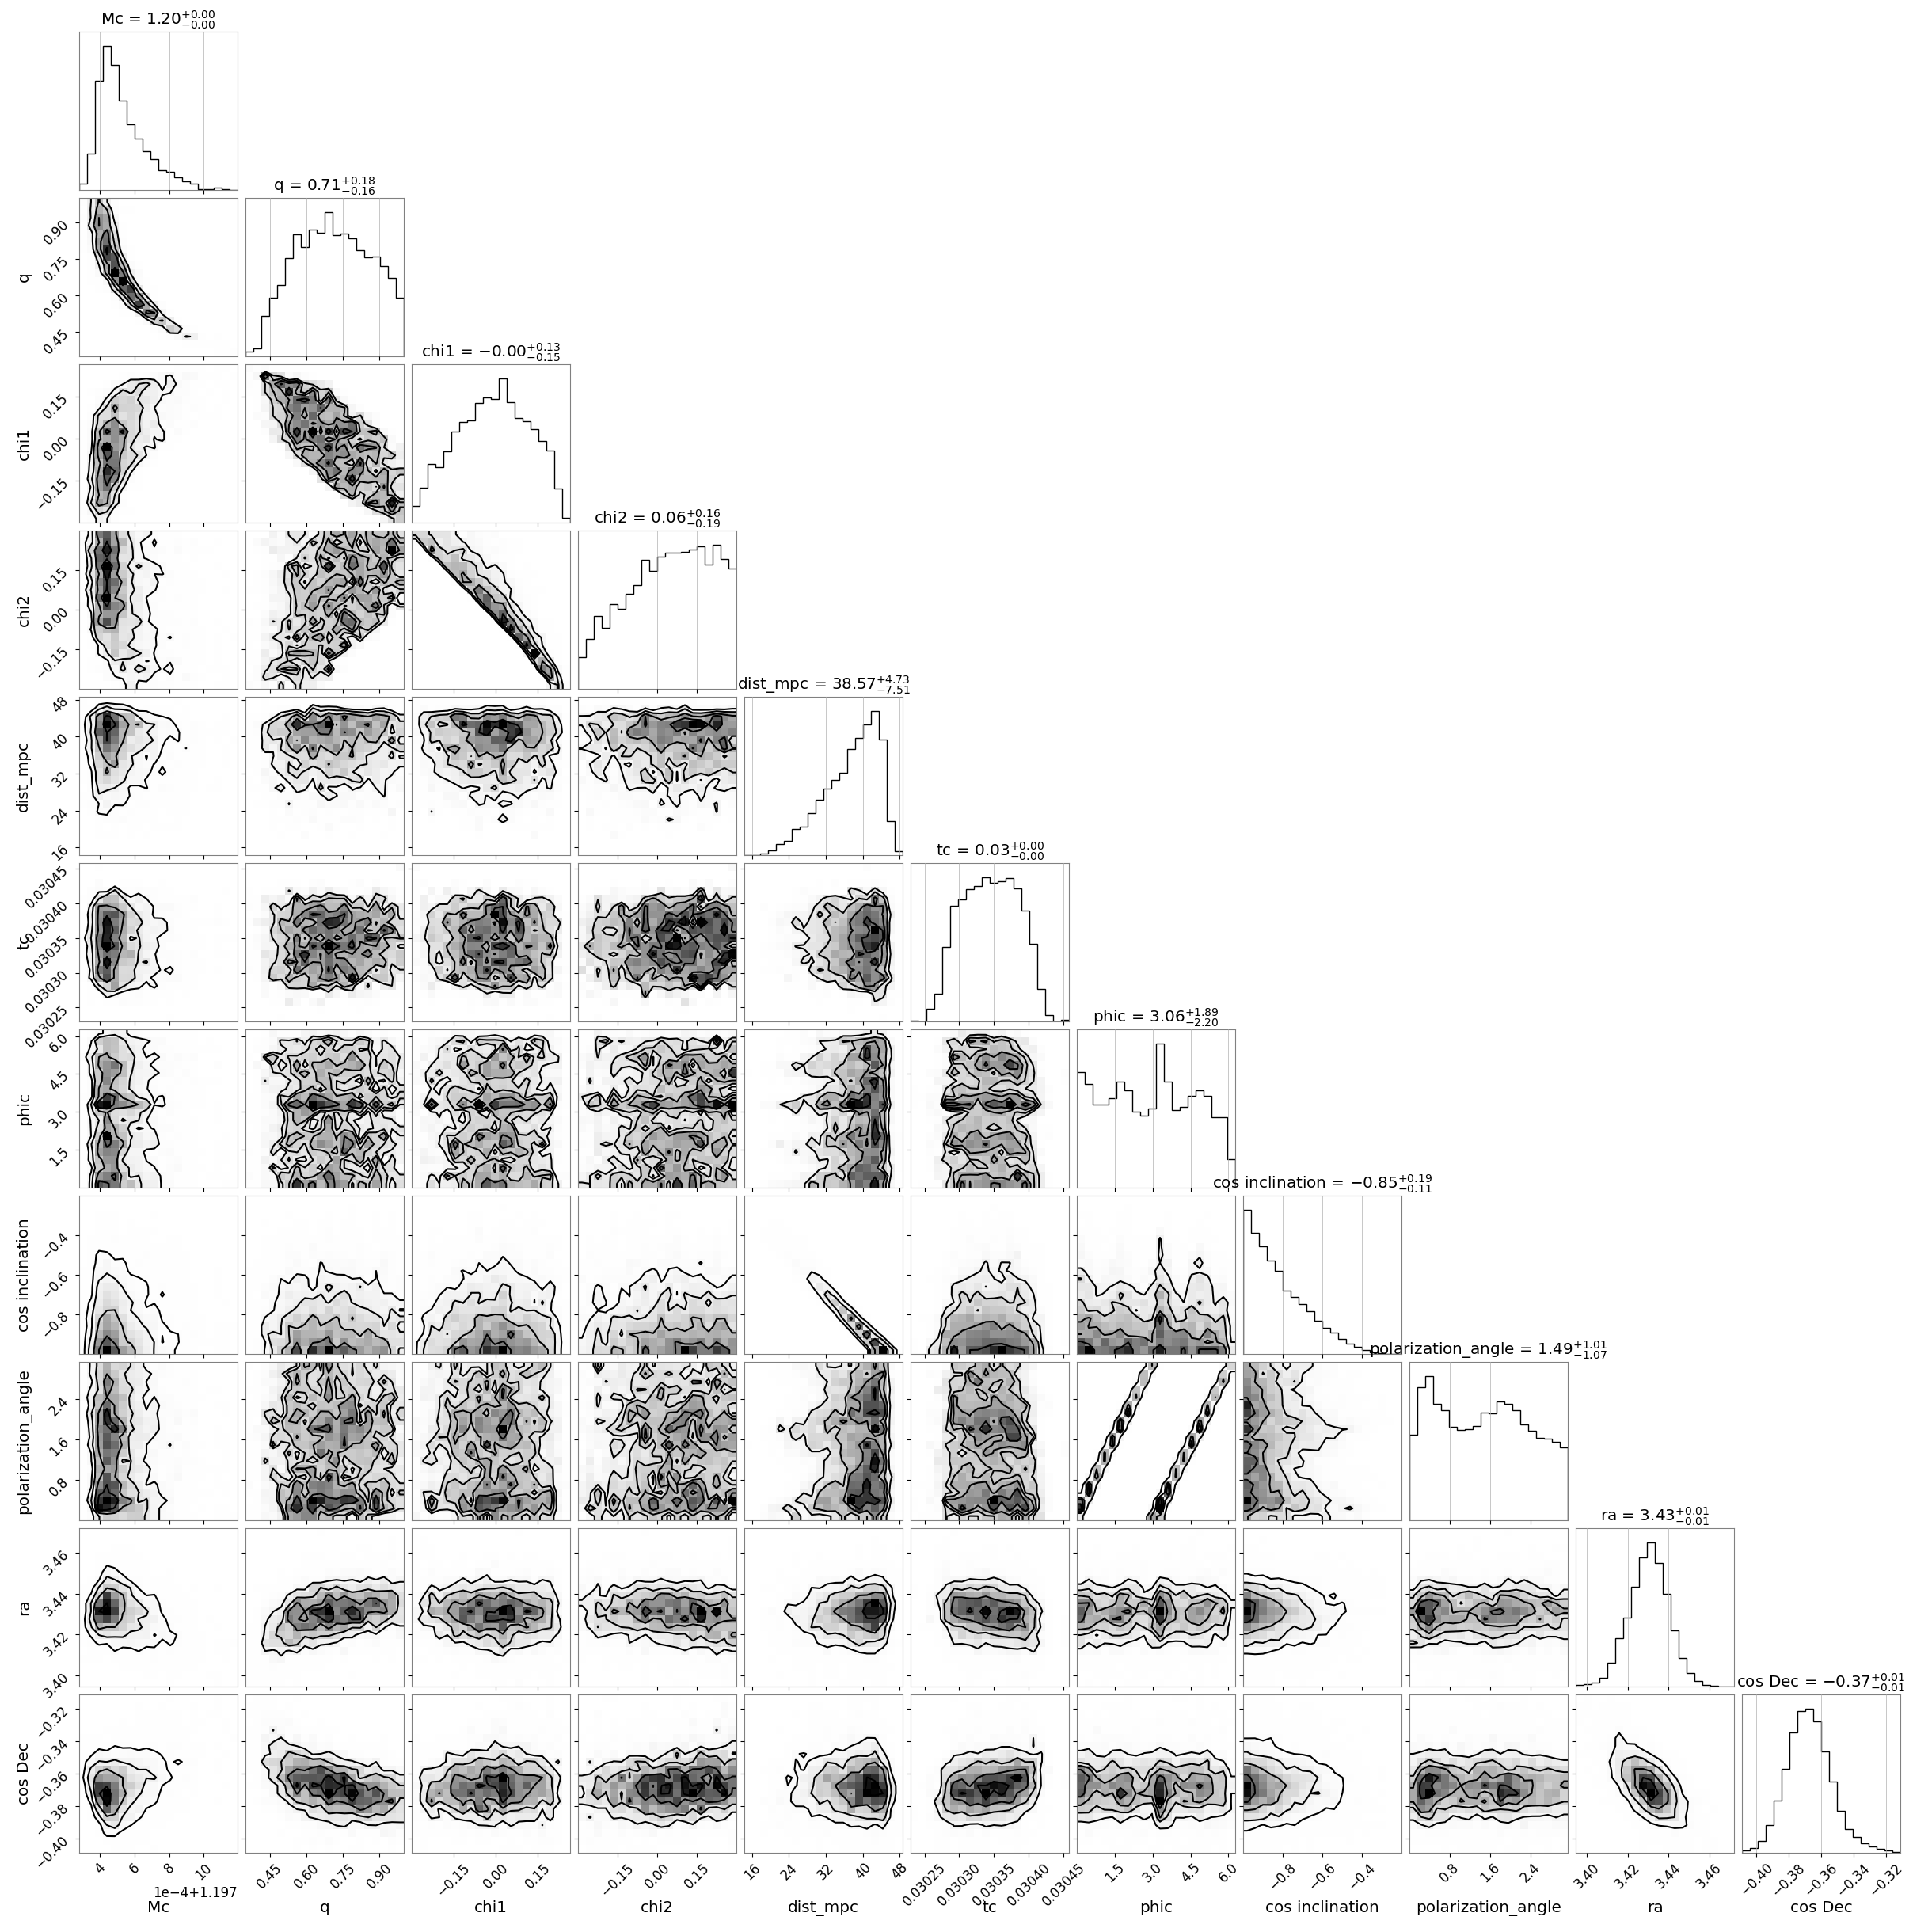
\includegraphics[width=0.99\linewidth]{static/GW170817.png}
\caption{
    hi
}
\label{fig:GW170817}
\end{figure}

Since we are using the \texttt{IMRPhenomD} waveform and the open data release
available on GWOSC \kw{cite} does not provide the posterior samples for this
waveform, we run Bilby using the same prior and waveform model as a reference
for comparison. From fig \ref{fig:GW150914} and \ref{fig:GW170817}, we can see
the 11-dimensional posteriors results produced by our pipeline are consistent
with the results obtained using Bilby \kw{cite}.

% Describe the distance between flowMC result and Bilby result using
% Jensen-Shannon divergence, scipy has a function to compute that in
% scipy.spatial.distance

For a quantitative comparison between results obtained through our code and
other existing tools, we compute the Jensen-Shannon divergence of the
marginalized distribution between our code and \texttt{Bilby}. The
Jensen-Shannon divergence is a symmetric measure of the distance between two
probability distributions, with a value of 0 indicating identical distributions
and a value of $\ln{2} \textrm{nat}$ representing the maximum possible
divergence between two distributions.
\kw{Report JSO} 

\section{Discussion}
\label{sec: Discussion}

% Brief summary
In this work, we present a PE pipeline for GW events that is efficient and
flexible. With differentiable waveform models, heterodyned likelihood and
normalizing flow enhanced sampler \texttt{flowMC}, we can estimate the
parameters of GW150914 and GW170817 in \kw{Quote speed}. Our method is general
and extensible, \kw{continue}.

% Compared to other works
There are recent works from different groups on speeding up parameter estimation
of gravitational wave, including efficient reparameterization and deep learning
\kw{cite}. While all of these methods can get down to minutes-scale parameter
estimation with high fidelity, we would like to highlight the unique strength of
this work, and the potential interplay between our work and others' work.

% Stephen's work
Compared to \kw{Stephan's paper}, we do not rely on pre-training the neural
network on a large collection of waveforms and noise realization. This means as
soon as new waveform models and noise models are available, our algorithm can
already be deployed. Furthermore, our method is essentially an MCMC algorithm,
which inherits the merit of convergence measures in MCMC. As we are only using
the normalizing flow as a proposal distribution, and the normalizing flow is
trained jointly with a local sampler, we do not suffer from overfitting since
our training data is being generated on the fly and is always approaching the
target distribution. In this sense, we do not introduce potential extra
systematic error to inference results.

While our pipeline uses the sample generated by the local sampler for training,
one can also supply a pre-trained normalizing flow model to our pipeline to
bypass the training stage. This can further reduce the total runtime of our
inference pipeline. However, this may introduce potential systematic bias in the
inference result if the pre-trained network is not able to capture the
complexity presented in the data.

%Tousif's work
Compared to \kw{Tousif's paper}, we do not rely on handcrafted
reparameterization of the coordinate systems. If the reparameterization scheme
is known ahead of time, a nice reparameterization is also encouraged. However,
handcrafted reparameterization depends on the assumptions used in deriving the
reparameterization scheme, which would inevitably run into limitations of use
cases. Our work can be viewed as an automatic reparameterization powered by
normalizing flow, while not being exact hence as efficient as an explicit
reparameterization, the method proposed in this work applies to a much
border class of problems, such as parameter estimation with precessing
waveforms, testing GR, and multi-event joint inference.

It is always beneficial to reparameterize if the reparameterization is known
ahead of time. For the class of problems where \kw{Tousif's paper} applies, we
can incorporate the reparameterization scheme into our MCMC pipeline to reduce
the complexity of the problem, hence speeding up the training phase. On the
other hand, if there is part of the target posterior that is not included in the
reparameterization scheme, the normalizing flow should still be able to learn to
produce accurate samples efficiently.

The two relevant works represent two orthogonal directions one can take in
building next generation tools in general. On one hand, there are modern tools
such as deep learning that are very flexible and powerful, but may need to rely
on having highly robust training data. On the other hand, there are traditional
tools that make use of our understanding of the underlying physics to simplify
the problem, which relies on having good intuition of the problem. Both
approaches rely on having a somewhat reasonable prior on how to approach the
problem. The main difference between methods used in industrial products and
scientific problems is scientific problems often try to address questions one
may have not been answered before, hence it is supposed to be far away from our
prior knowledge, meaning one need to take capability to generalize beyond the
current problem into account while building the tool. Our work utilizes both
reparameterization and deep learning, yet our method can be trivially extended
to problems beyond standard GW analysis that reparameterization or deep learning
alone may have trouble dealing with. We believe such flexibility is crucial for
building scientific tools.

% Additional traits for having differentiable waveforms
There are some future developments we are working on. While IMRPhenomD is
a reasonable start, it lacks some qualitative features that other
state-of-the-art models have, such as precession, higher mode, and eccentricity \kw{cite}. It
also has a higher mismatch with reference numerical relativity waveforms compared
to more recent waveform models. Currently, we are working on building differentiable
IMRPhenomPv2 and NRSurrogate waveforms. Going forward, we encourage the waveform
development community to leverage autodiff environments such as Jax when
constructing new waveform models. Having a differentiable waveform model is not
only beneficial for parameter estimation, but also for other applications such
as calibrating waveforms to numerical relativity results, as detailed in
\kw{cite}.

% Access to higher dimensional problem
While standard GW analysis goes up to 17 dimensions. non-standard GW PE problems
can have more parameters, which could potentially lead to more complicated
geometry in the target posterior that is hard to reparameterize. For example,
there are \kw{Be specific with the number} parameterized modifications to the
waveform one can introduce when testing GR, which means there are \kw{the number}
extra parameters one would need to consider in the PE process. Worse, these
parameters often introduce non-trivial degeneracies such as local correlation
and multi-modality. Currently testing GR is limited to varying these
modifications one at a time, partially due to the bottleneck in the sampler. Given
the gradient-based and normalizing flow-enhanced sampler, our code shows
the potential in solving this problem in full at once.


% Other detectors configuration

To perform realistic PE with our pipeline, the antenna pattern of the
detector network needed to be taken into account. Our current code can perform
parameter estimation for any combination of the Hanford, Livingston, and Virgo
detectors, under the assumption of short signals such that the effect of Earth's
rotation can be ignored. For next-generation detector networks such as the
Einstein Telescope and the Cosmic Explorer \kw{cite}, a differentiable version
of their antenna pattern is needed.

% More features such as marginalization
The features we have implemented are the barebone version of parameter
estimation. We do not include marginalization schemes such as time, phase, and
calibration lines marginalization. Because of the reasonable performance of the sampler on
accelerators, time and phase marginalization is not necessary, as the
performance of our implementation is not significantly impacted by having two
extra dimensions. Other marginalization modes should be considered in the future.

% JIT overhead
Jax's JIT compilation drastically reduces the computational time to evaluate the
likelihood. However, it comes with a compilation overhead when the likelihood is
evaluated for the first time. We observe that the compilation time could depend
on the device where the code will be run. This is expected since Jax leverage
Accelerated Linear Algebra (XLA) takes advantage of accelerators, which means
Jax needs to compile the code for the specific device according to its
architecture. On an Nvidia A100 GPU, the compilation overhead could go up to 5
minutes for the waveform we are using. For the cases we have studied, the time
needed to obtain converging results on an A100 is about 2-3 minutes. This means
the compilation overhead is dominating the wall-clock time of the specific PE
run we considered. To utilize our implementation to its full potential, we are
looking into ways to reduce the compilation overhead or to cache the
compilation results to avoid paying the compilation overhead for every event.

% Faster maximum likelihood finder

Another overhead we are looking into reducing is the time needed to find the
reference waveform for heterodyning the likelihood. Currently, we are using
\texttt{differential evolution} available in \texttt{scipy} to find the waveform
parameters which maximize the likelihood. Since \texttt{differnetial evolution}
has not been implemented in Jax, and the Jax waveform we use is not compatible
with the parallelization scheme in the \texttt{scipy} library, it takes around 5
minutes \kw{Benchmark it in the code and make this number precise.} to find the
reference waveform parameters for GW170817. There are two ways to improve the
performance in finding the parameters of the reference waveform. First, we can
explore different optimization strategy that is more compatible with the
strength of our pipeline, in particular differentiability of our likelihood and
the possibility to evaluate many waveforms in parallel with a GPU. Particle
swarm or stochastic gradient descent methods are promising candidates which we
intend to investigate in the future. 

Another way to reduce the time of finding the maximum likelihood waveform is to
incorporate marginalization of extrinsic parameters to reduce the dimensionality
of the optimization problem. Currently, we simultaneously maximize all 11 GW
parameters, which is unnecessarily complicated and expensive. There are
long-existing marginalization schemes over extrinsic parameters such as the merger
time and phase, which can find the corresponding maximum likelihood waveform
much more efficiently when compared to differential evolution. We expect
implementing these marginalization schemes will reduce the time needed to find
the reference waveform parameters by obtaining the extrinsic parameters and by
reducing the dimensionality of the optimization problem for the intrinsic
parameters.

% Multi-device scaling
One important aspect of modern computing is scalability, meaning it is generally
favorable if one can simply put more computing units in the same problem and
reduce the Wall time. In our case, this means we would like to use more than one
GPU for the same PE process. More GPUs can help in the following ways: first,
more GPUs means we can run more independent chains at the same time, which can
generate more samples faster. But more importantly, as shown in this work and
\kw{cite flowMC?}, more independent chains also help with reducing the burn-in
time. Parallelizing over the number of chain dimension is trivial and does not
require much change to the current infrastructure. Another way more GPUs can
helps is by allowing faster training of larger flow models. While the training time
is not the biggest bottleneck given the flow model used in this study, more GPUs
means we can increase the bandwidth of the flow model by increasing its size
while keeping the training time the same. This helps capture more complex
geometry in the target space, which can lead to more accurate results in general.


\section{Acknowledgements}
Thanks Will.

\bibliography{bib}

\end{document}
